\documentclass[preprint,12pt,times]{elsarticle}

%% Use the option review to obtain double line spacing
%% \documentclass[preprint,review,12pt]{elsarticle}

%% Use the options 1p,twocolumn; 3p; 3p,twocolumn; 5p; or 5p,twocolumn
%% for a journal layout:
%% \documentclass[final,1p,times]{elsarticle}
%% \documentclass[final,1p,times,twocolumn]{elsarticle}
%% \documentclass[final,3p,times]{elsarticle}
%% \documentclass[final,3p,times,twocolumn]{elsarticle}
%% \documentclass[final,5p,times]{elsarticle}
% \documentclass[final,5p,times,twocolumn]{elsarticle}

%% if you use PostScript figures in your article
%% use the graphics package for simple commands
%% \usepackage{graphics}
%% or use the graphicx package for more complicated commands
%% \usepackage{graphicx}
%% or use the epsfig package if you prefer to use the old commands
%% \usepackage{epsfig}

%% The amssymb package provides various useful mathematical symbols
\usepackage{amssymb}
%% The amsthm package provides extended theorem environments
%% \usepackage{amsthm}

%% The lineno packages adds line numbers. Start line numbering with
%% \begin{linenumbers}, end it with \end{linenumbers}. Or switch it on
%% for the whole article with \linenumbers after \end{frontmatter}.
\usepackage{lineno}

\biboptions{sort&compress}

\usepackage{amsmath}
\usepackage{textcomp} %Permet d'introduire un mu droit à l'aide de \textmu en dehors de l'environnement math

%\usepackage[leftbars]{changebar} %Pour insérer une barre de mise à  jour (à  gauche car [leftbars]) au moyen de \begin{changebar} %Ne fonctionne pas pour passer du DVI au pdf -> utiliser DV -> PS -> pdf %Ne fontionne pas avec figure* et table*

\usepackage{multirow}
%\usepackage{rotating} %Pour effectuer la rotation d'un tableau à  l'aide de "\begin{sidewaystable} et \end{}" et supprimer "\begin{table} et \end{}"
\usepackage{pdflscape}
\usepackage{tikz}
\usetikzlibrary{patterns}
\usepackage{pgfplots}
\usepackage{accents}

\usepackage{dblfloatfix} % fix for bottom-placement of figure*

%\newcommand{\e}[1]{\exp\left({#1}\right)}
\newcommand{\e}[1]{\mbox{\ensuremath{\mathrm{e}^{#1}}}}
\DeclareMathOperator{\sigmoid}{sig}
\newcommand{\lay}[1]{^{(#1)}}
\newcommand{\dotp}{\boldsymbol{\cdot}}
\newcommand{\w}{\mbox{\large\ensuremath{\mathsf{w}}}}
\newcommand{\mdot}[1]{\accentset{\mbox{\bfseries .}}{#1}}

%%%%%%%%%%%%%%%%%%%%%%%%%%%%%%%%%%%%%%%%%%%%%%%%%%%
% To insert highlighted comments with author's name
% Adapted from https://www.willusher.io/latex/2018/07/10/comments-in-latex
\usepackage{soul} %Can also be used to highlight text with \hl{highlighted text}
\usepackage{color}
\definecolor{VWpink}{RGB}{255,113,206} % VaporWave color palette
\definecolor{VWblue}{RGB}{1,205,254} % VaporWave color palette
\definecolor{VWgreen}{RGB}{5,255,161} % VaporWave color palette
\definecolor{VWviolet}{RGB}{185,103,255} % VaporWave color palette
\definecolor{VWyellow}{RGB}{255,251,150} % VaporWave color palette
% We also use DeclareRobustCommand instead of
% NewCommand so that the command will work in captions
% and other contexts as well.
\DeclareRobustCommand{\FD}[1]{ {\begingroup\sethlcolor{VWgreen}\textcolor{black}{\hl{[FD:] #1}}\endgroup} }
\DeclareRobustCommand{\OP}[1]{ {\begingroup\sethlcolor{VWblue}\textcolor{black}{\hl{[OP:] #1}}\endgroup} }
% The highlight comment command can then be used in the text: \FD{This is an example comment!}
%%%%%%%%%%%%%%%%%%%%%%%%%%%%%%%%%%%%%%%%%%%%%%%%%%%


\journal{CIRP Journal of Manufacturing Science and Technology}

\begin{document}

%%%%%%%%%%%%%%%%%%%%%%%%%%
\begin{frontmatter}

\title{Predictive 3D modelling of free oblique cutting of Ti6Al4V titanium alloy and experimental validation for a wide range of conditions\\ \FD{Include AI?}}

\author[1]{F. Ducobu\corref{cor1}}
\ead{Francois.Ducobu@umons.ac.be}
\cortext[cor1]{Corresponding author. Tel.: +32 65 45 68}

\author[2]{O. Pantal\'{e}}
\author[3]{B. Lauwers}

\address[1]{Machine Design and Production Engineering Lab, Research Institute for Science and Material Engineering, UMONS, Belgium}
\address[2]{Laboratoire G\'{e}nie de Production, INP/ENIT, Universit\'{e} de Toulouse, Tarbes, France}
\address[3]{Department of Mechanical Engineering, KU Leuven \& Flanders Make@KU Leuven-MaPS, Belgium}

%%%%%%%%%%%%%%%%%%%%%%%%%%
\begin{abstract}

Modelling of the cutting process needs to move from a 2D to a 3D configuration to get closer to industrial applications. The study introduces a predictive 3D finite element model of free orthogonal and oblique cutting with an ANN-based material constitutive model and experimental validation in strictly the same conditions (cutting and geometrical). Predictive performance of the model is high for the forces in the 3 directions and the chip thickness ratio on all 36 cutting conditions (including 2 inclination angles). Accuracy of the main cutting force is excellent: the mean difference with the experiments is 3\%.

\FD{Review and update}

\end{abstract}
%%%%%%%%%%%%%%%%%%%%%%%%%%

%%%%%%%%%%%%%%%%%%%%%%%%%%
\begin{keyword}
%% keywords here, in the form: keyword \sep keyword

Oblique cutting \sep Finite element method (FEM) \sep Predictive model \sep Artificial Neural Network (ANN)

\end{keyword}
%%%%%%%%%%%%%%%%%%%%%%%%%%

\end{frontmatter}
%%%%%%%%%%%%%%%%%%%%%%%%%%

%%
%% Start line numbering here if you want
%%
\linenumbers

%% main text
%%%%%%%%%%%%%%%%%%%%%%%%%%
\section{Introduction}
\label{Intro}
%%%%%%%%%%%%%%%%%%%%%%%%%%

Selection of the tools and the cutting conditions in machining, but also comprehension of the influence of the process parameters on the quality of a component and its optimisation, are still difficult to achieve because of the high level of complexity and linked nonlinear phenomena. In the frame of digital manufacturing and Industry 4.0, modelling of the cutting process supports them, while remaining a challenging task. As highlighted by Arrazola et al. \cite{arrazola_Recent_2013}, most finite element (FE) models are developed in 2D (orthogonal cutting configuration usually) although industrial applications require a 3D modelling.

Experimental validation of a model is a crucial step in the modelling of the cutting process. The experimental configuration must be as close as possible to the simulation. For orthogonal cutting validation, a rotating movement usually generates the cutting speed. This is often achieved in turning \cite{agmell_Development_2018} or in milling \cite{xu_Simulation_2021} and the diameter of the rotating part must be large enough to reduce the influence of the curvature on the results. Experimental configurations in strictly orthogonal cutting conditions are less often adopted, for example, in broaching \cite{abouridouane_Friction_2021} or milling \cite{ducobu_Experimental_2015, sela_Measurement_2021} machines. While they remove assumptions linked to the rotating cutting movement, they usually allow for lower cutting speeds (except on a dedicated machine, such as in Afrasiabi et al. \cite{afrasiabi_NumericalExperimental_2021}). Free oblique cutting with a straight cutting edge has not been studied yet: all the efforts have been focussing on orthogonal cutting (mostly for 2D validation).

Lagrangian and Eulerian formulations are the most used for FE modelling of the cutting process. Combinations of formulations, such as Arbitrary Lagrangian-Eulerian (ALE) and Coupled Eulerian-Lagrangian (CEL) are increasingly used to avoid (or reduce) mesh distortions \cite{ducobu_Application_2016}. The Coupled Eulerian-Lagrangian (CEL) formulation has recently been successfully applied to the modelling of cutting (2D orthogonal configuration): it provides accurate results with a realistic chip shape and no mesh distortion \cite{ducobu_Application_2016}. First applications in 3D are found in recent works \cite{xu_Simulation_2021, ducobu_Finite_2017, ambrosio_New_2022, vovk_Finite_2020, hardt_Three_2021}. They cover (free) orthogonal cutting or a simple 3D operation, while free oblique cutting still needs to be investigated.

The behaviour of the machined material is one of the key aspects of a FE model \cite{arrazola_Recent_2013, melkote_Advances_2017}. Research is very intense in this field, which leads to a growing number of material constitutive models ranging from empirical to physical models, some including microstructure effects \cite{melkote_Advances_2017}. The thermo-elasto-viscoplastic empirical model of Johnson-Cook (JC) \cite{johnson_Constitutive_1983} is still the most used so far:
%
\begin{equation}\label{eq:J-C}
	\sigma^{y} = \left(A + B\ \varepsilon^{p^n} \right) \left(1 + C\ \ln\frac{{\dot{\varepsilon}}^p}{\dot{\varepsilon}_{0}^{p}}\right) \left(1 - \left[\frac{T - T_{\text{room}}}{T_{\text{melt}} - T_{\text{room}}}\right]^{m}\right)
\end{equation}
%
The flow stress, $\sigma^{y}$, is a function of the plastic strain, $\varepsilon^{p}$, of the plastic strain rate, ${\dot{\varepsilon}}^{p}$, and of the temperature, $T$. It is composed of 3 terms describing independently plastic, viscous and thermal aspects. One of the points in favour of its adoption is the rather limited number of parameters to be identified, 5: $A$, $B$, $C$, $m$ and $n$. $\dot{\varepsilon}_{0}^{p}$ is the reference plastic strain rate, while $T_{\text{room}}$ and $T_{\text{melt}}$ are the room temperature and the melting temperature, respectively. More recent models developed based on it, such as the one of Calamaz et al. \cite{calamaz_New_2008}, increase this number of parameters (for Calamaz's particular model to 9). The better (in theory) description of the behaviour is achieved at the cost of greater complexity of the identification process and of a reduction of the link with the physical meaning of the model.

One issue of material behaviour modelling for cutting simulation is the identification of the model parameters, moreover as the experimental equipment does not allow to reach the high levels of strains, strain rates and temperature of machining \cite{melkote_Advances_2017}. Inverse identification is an alternative, but the uniqueness of the solution is not always guaranteed \cite{arrazola_Recent_2013, melkote_Advances_2017}. The early work of Özel and Altan \cite{ozel_Determination_2000} used  the least squares method to inversely identify the input parameters of a FE model. Shrot and Bäker \cite{shrot_Determination_2012} then used the Levenberg–Marquardt algorithm for their identification of the constitutive material parameters. They showed that similar results (cutting forces and chip morphology) could be obtained by different sets of parameters and therefore highlighted the non-uniqueness of the solution of the inverse problem. In addition to the flow stress parameters, Klocke et al. \cite{klocke_Orthogonal_2013} also identified the damage parameters. In more recent works, such as Bosetti et al. \cite{bosetti_Identification_2013} and Denkena et al. \cite{denkena_Inverse_2015}, the approach to tackle the inverse identification problem is moving from optimisation to Artificial Intelligence (AI) based methods. The Downhill Simplex Algorithm (DSA) is adopted by Bergs et al. \cite{bergs_Determination_2020} and by Hardt et al. \cite{hardt_Investigations_2021} for AISI 1045. Stampfer et al. \cite{stampfer_Material_2021} also selected the DSA when dealing with AISI 4140 tempered at 3 different temperatures. In \cite{hardt_Application_2021}, Hardt et al. showed that the Particle Swarm Optimization (PSO) was more efficient to solve the inverse problem than the Downhill Simplex Algorithm, even if computation time is still significant. In an effort to reduce it, an Efficient Global Optimization (EGO) algorithm has recently been introduced by Kugalur Palanisamy et al. \cite{kugalurpalanisamy_Identification_2022}. They simultaneously identified the parameters of the material constitutive model and of the friction model for Ti6Al4V. Most of these works highlight the non-uniqueness of the identification and they all require the definition of the analytical expression of the constitutive model.

This paper fills the literature gap on oblique cutting by investigating free orthogonal and oblique 3D cutting configurations from both the experimental and the numerical points of view. An Artificial Neural Network (ANN), introduced in Pantalé et al. \cite{pantale_Efficient_2022}, is implemented in a FE cutting model for the first time instead of the analytical JC law. A broad range of cutting speeds (6), uncut chip thicknesses (3) and inclination angles (2) resulting in 36 different conditions are considered to demonstrate the predictive ability of the FE model for fundamental variables. The main goals of a predictive model are the accurate modelling of the trends of the results when the conditions change and predicted values in good agreement with the experimental ones (exact values are not looked for due to experimental dispersions). This type of models aims at supporting future choices and developments without the need of experimental data. No assumption is made about the geometry of the machined workpiece in the model (i.e. its width is the same as in the experiments), while keeping computation time relevant for industrial applications. The developments apply to the titanium alloy Ti6Al4V.

%%%%%%%%%%%%%%%%%%%%%%%%%%
\section{Experimental setup}
\label{ExpSet}
%%%%%%%%%%%%%%%%%%%%%%%%%%

A 3-axis GF Mikron VCE 600 Pro milling machine is used to carry out dry free orthogonal and oblique cutting tests on Ti6Al4V (grade 5 annealed at 750\textdegree{}C for 1 h followed by air cooling) with the same kinematics as a shaper. As shown in Figure \ref{ExpSetup}, the tungsten carbide tool (modified LCGN160602-0600-FG, CP500 from SECO) is fixed on a dedicated holder (modified CFHN-06 from SECO) and the sample to be cut is clamped in the spindle (no rotation is allowed during the test). The top of the sample includes 3 ribs of 1 mm in width (width of the tool is 6 mm) and 10 mm in length. The test consists of removing the upper layer (its height is the uncut chip thickness, $h$) of one rib at the prescribed cutting speed, $v_c$. The cutting speed is provided by the feed rate, $v_f$, of the machine (max. value of 40 m/min). The tool cutting edge inclination, $\lambda_s$, results from the relative angular orientation of the tool and the sample. Table \ref{tab:CutCond} shows the cutting conditions: 6 cutting speeds, 3 uncut chip thicknesses and 2 inclination angles, each is repeated 3 times.

\begin{figure}[!h]
\centering
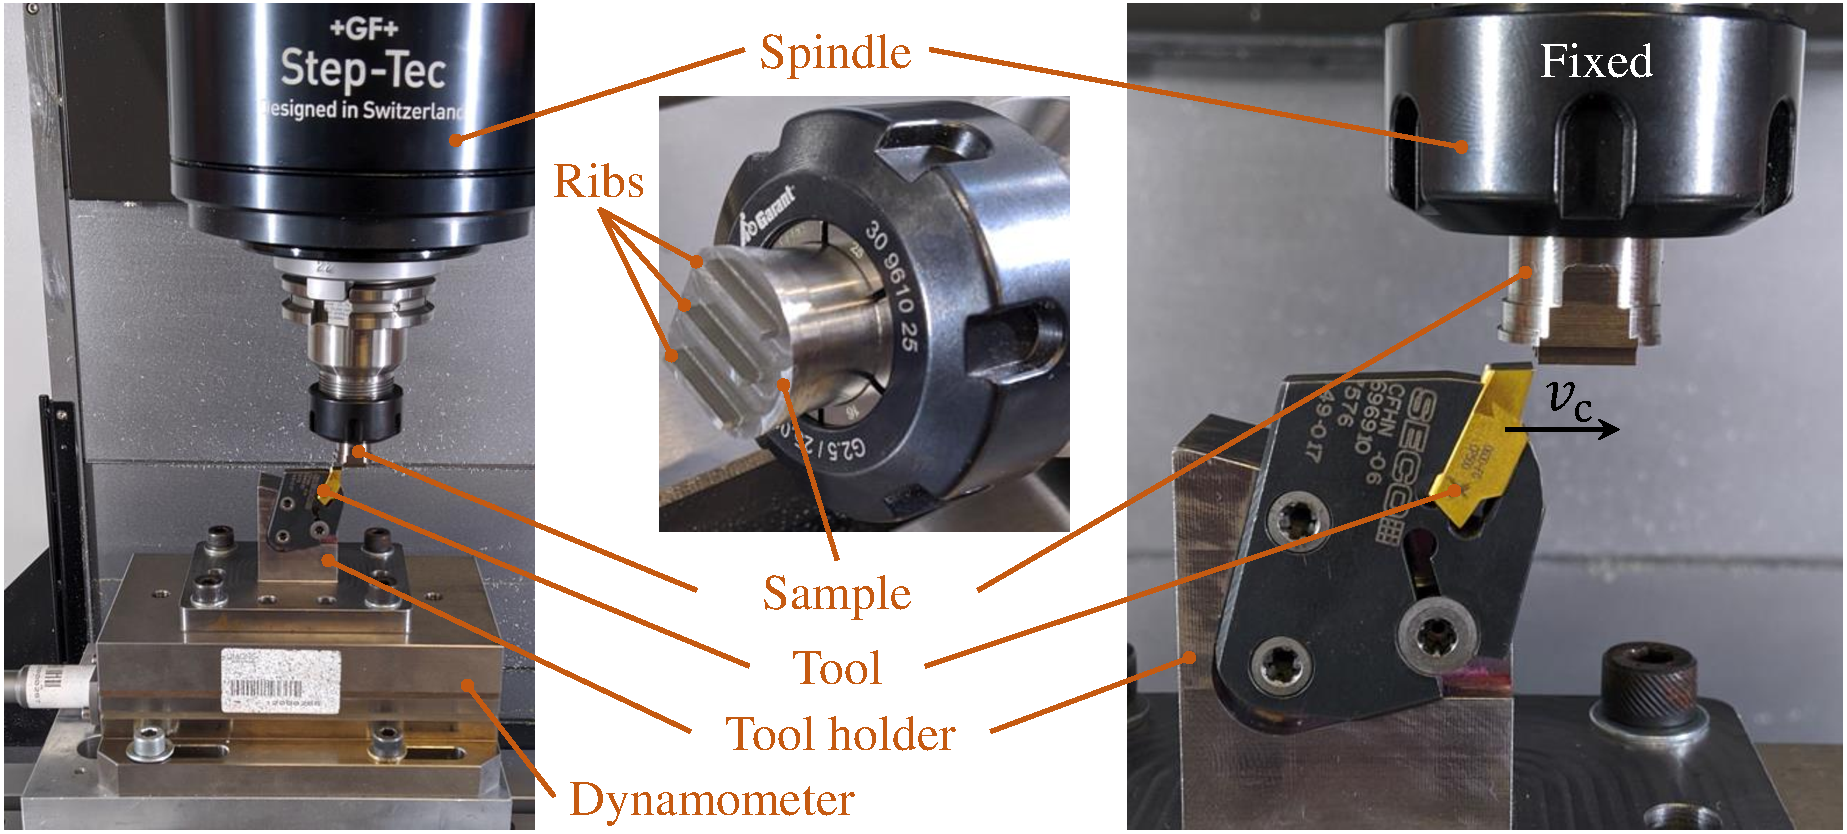
\includegraphics[width = 140 mm]{Figures/ExpSetup} % 140 mm, 1.5\columnwidth
\caption{Experimental setup}
\label{ExpSetup}
\end{figure}

%
\begin{table}[!h]
\begin{center}
\caption{\label{tab:CutCond} Cutting conditions of the study}
\begin{tabular}{ll}
\hline\noalign{\smallskip}
Parameter  & Values\\
\noalign{\smallskip}\hline\noalign{\smallskip}
Cutting speed, $v_c$ (m/min) & 5, 7.5, 10, 20, 30, 40\\
Uncut chip thickness, $h$ (\textmu{}m) & 40, 60, 80\\
Cutting edge inclination, $\lambda_s$ (\textdegree{}) & 0, 6\\
Width of the workpiece (mm) & 1\\
Length of the workpiece (mm) & 10\\
Width of the cutting edge (mm) & 6 (1.1 in the model)\\
Cutting edge radius, $r_\beta$ (\textmu{}m) & 20\\
Rake angle, $\gamma_0$ (\textdegree{}) & 15\\
Clearance angle, $\alpha_0$ (\textdegree{}) & 2\\
\noalign{\smallskip}\hline
\end{tabular}
\end{center}
\end{table}
%

Forces are measured with a 3-component Kistler 9257B dynamometer and are amplified by a Kistler 5070A charge amplifier. Acquisition is performed at 3 kHz with a Kistler 5697A2 data acquisition system and the DynoWare software. Recorded forces are then filtered with a second-order low-pass Bessel filter at 750 Hz before computing the mean value of the signal at steady state.

All the chips are collected and observed with a Dino Lite digital microscope AM7013MZT (5 MP, magnification $20\times$ -- $250\times$). Each chip is measured 3 times along its length to get a mean value representative of the whole chip.


%%%%%%%%%%%%%%%%%%%%%%%%%%
\section{Finite element model}
\label{FEM}
%%%%%%%%%%%%%%%%%%%%%%%%%%

\subsection{Modelling choices}

The CEL formulation is adopted to model the dry free orthogonal and oblique cutting tests with Abaqus/Explicit 2020. The 3D model is composed of a fixed Lagrangian tool and a Eulerian workpiece (Figure \ref{BC}). Chip formation occurs by plastic flow across the Eulerian domain with no mesh distortion. The Eulerian formulation enables to form chips without damage properties, removing modelling assumptions. These two characteristics contribute to cutting models providing accurate results and realistic chips \cite{ducobu_Application_2016}.

\begin{figure}[!h]
\centering
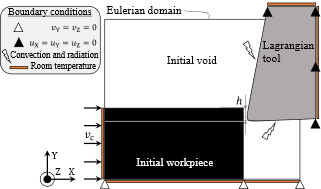
\includegraphics[width = 140 mm]{Figures/BC} % 90 mm, \columnwidth
\caption{Boundary conditions and schematic initial geometry of the model}
\label{BC}
\end{figure}

As shown in Figure \ref{FEConfig}, the full width of the workpiece, i.e. a rib in the experiments, (1 mm) is modelled. To allow chip formation and side flow, the Eulerian domain is wider (it includes the volume in which material can move). The volume above the initial workpiece is also meshed with Eulerian elements for the same reasons. As in the experiments and to fulfil the hypothesis of free orthogonal and oblique cutting, the tool is wider than the workpiece (it is of 1.1 mm in the model and of 6 mm in the experiments). It is very important to stress that the models are the same for both inclination angles: they only differ by the rotation of the tool of 6\textdegree{} about Y axis as in the experiments (Figure \ref{FEConfig}). This, coupled to the absence of assumptions when developing the models, contributes to make the models predictive: no input is changed when cutting conditions do.

\begin{figure}[!h]
\centering
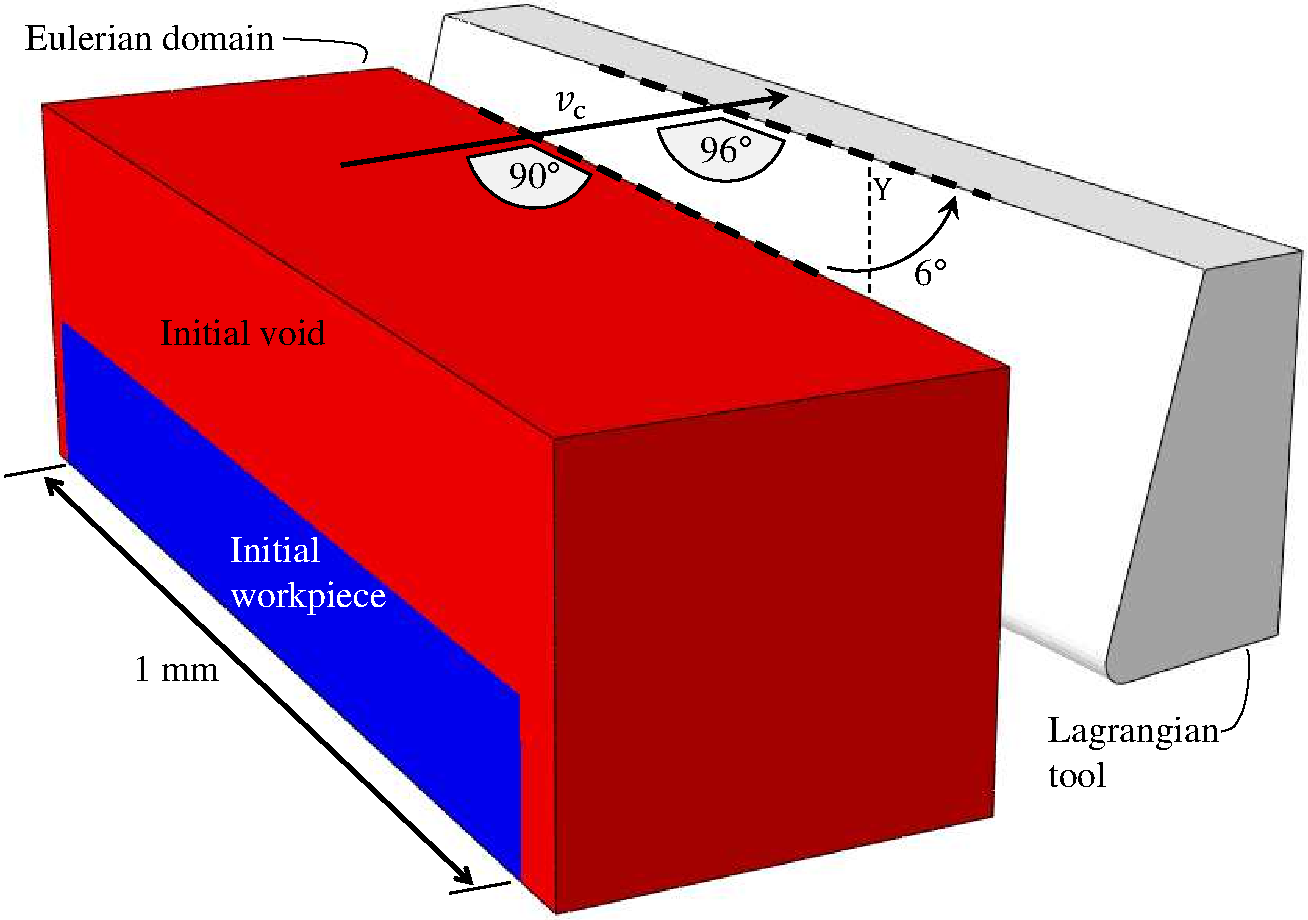
\includegraphics[width = 140 mm]{Figures/FEConfig}
\caption{Configuration of the FE model for $\lambda_s$ = 6\textdegree{}}
\label{FEConfig}
\end{figure}

According to a previous mesh sensitivity study in orthogonal cutting with the CEL formulation \cite{ducobu_Finite_2017}, elements edge size is 5 \textmu{}m in the plane parallel to the cutting speed. In the direction perpendicular to this plane, it is 5 \textmu{}m in areas close to the lateral boundaries of the Eulerian domain and 50 \textmu{}m in the middle of the workpiece. To reduce computation time, the size of the model depends on the value of the uncut chip thickness. This results in a Eulerian domain (EC3D8RT linear 3D Eulerian elements with 8 nodes, coupled mechanical-thermal behaviour and reduced integration) composed of 216,550 to 273,350 nodes and a Langrangian domain (C3D8T linear 3D Lagrangian elements with 8 nodes, coupled mechanical-thermal behaviour) of 4,650 nodes.

The Ti6Al4V workpiece is assumed to be thermo-elasto-viscoplastic (isotropic) and inelastic heat fraction is 0.9. JC set of parameters from Seo et al. \cite{seo_Constitutive_2005} is adopted as the value of $A$ corresponds to the typical yield stress value of Ti6Al4V and this set proved to provide the best results among 20 sets available in the literature \cite{ducobu_Importance_2017}.  The tungsten carbide tool with TiN coating is assumed to be linear elastic. Material properties are provided in Table \ref{tab:prop}.

%
\begin{table}[!h]
\begin{center}
\caption{\label{tab:prop} Materials properties \cite{seo_Constitutive_2005, _GRANTA_2020, milosevic_Thermophysical_2012}}
\begin{tabular}{lll}
\hline\noalign{\smallskip}
Young's modulus, $E$ (GPa) & Ti6Al4V & 113.8$^*$\\
 & WC & 650\\
Poisson's ratio, $\nu$ & Ti6Al4V & 0.34\\
 & WC & 0.2\\
Density, $\rho$ (kg/m$^3$) & Ti6Al4V & 4,430\\
 & WC & 14,850\\
Conductivity, $k$ (W/mK) & Ti6Al4V & 6.3$^*$\\
 & WC & 100\\
Expansion, $\alpha$ (K$^{-1}$) & Ti6Al4V & 8.6 e$^{-6*}$\\
 & WC & 5 e$^{-6}$\\
Specific heat, $c_{p}$ (J/KgK) & Ti6Al4V & 531$^*$\\
 & WC & 202\\
\noalign{\smallskip}\hline\noalign{\smallskip}
JC constitutive model & $A$ (MPa) & 997.9\\
 & $B$ (MPa) & 653.1\\
 & $C$ & 0.0198\\
 & $m$ & 0.7\\
 & $n$ & 0.45\\
 & $\dot{\varepsilon}_{0}$ (s$^{-1}$) & 1\\
 & $T_{\text{room}}$ (K) & 293\\
 & $T_{\text{melt}}$ (K) & 1873\\
\noalign{\smallskip}\hline\noalign{\smallskip}
\end{tabular}
\end{center}
\vspace{-0.4cm}$^*$: Dependence to the temperature, value provided at 293 K
\end{table}
%

Following the experimental results of Rech et al. \cite{rech_Characterisation_2013}, Coulomb's friction is assumed to occur at the tool-workpiece interface and both friction, $\mu$, and heat partition, $\beta$, coefficients depend on the cutting speed. Limiting shear stress, $\tau_{\text{max}}$, is included and is given by
%
\begin{equation}
\tau_{\text{max}} = \frac{\text{yield stress}}{\sqrt{3}} = \frac{A}{\sqrt{3}}
\end{equation}
%
All the friction energy is converted into heat. Table \ref{tab:fricHeat} shows the friction coefficients adopted in this study.
%
\begin{table}[!h]
\begin{center}
\caption{\label{tab:fricHeat} Friction and heat transfer coefficients \cite{rech_Characterisation_2013, _GRANTA_2020}}
\begin{tabular}{lll}
\hline\noalign{\smallskip}
Cutting speed, $v_c$ (m/min) & $\mu$ & $\beta$\\
\noalign{\smallskip}\hline\noalign{\smallskip}
5 & 0.24 & 1\\
7.5 & 0.22 & 0.89\\
10 & 0.21 & 0.80\\
20 & 0.19 & 0.63\\
30 & 0.18 & 0.55\\
40 & 0.17 & 0.50\\
\noalign{\smallskip}\hline\noalign{\smallskip}
Limiting shear stress, $\tau_{\text{max}}$ (MPa) & 576\\
Convection, $U$ (W/m$^2$K) & 50\\
Radiation, $\epsilon$ & 0.3\\
\noalign{\smallskip}\hline\noalign{\smallskip}
\end{tabular}
\end{center}
\end{table}
%

Room temperature of 293 K is imposed on the upper and right surfaces of the tool and on the left and bottom surfaces of the workpiece (Figure \ref{BC}). Radiation and convection are assumed to occur on the rake and clearance faces of the tool. Initial temperature of the tool and the workpiece is set to room temperature (293 K). Heat transfer coefficients are provided in Table \ref{tab:fricHeat}.

\subsection{Material constitutive model of Ti6Al4V}

The constitutive model of the Ti6Al4V material used in all the numerical simulations proposed in section \ref{sec:ExpNumResults} is a thermo-elasto-viscoplastic law using a flow criterion based on an ANN identified for the selected material and implemented in the Abaqus/Explicit code via a Fortran routine VUHARD as proposed by Pantalé et al. in \cite{pantale_Efficient_2022}.
The principle of this approach consists in replacing the analytical formulation of the flow law, based on a Johnson-Cook or Zerilli-Armstrong type model, and allowing the calculation of the flow stress $\sigma^y$ as a function of the plastic strain $\varepsilon^p$, of the plastic strain rate, ${\dot{\varepsilon}}^p$, and of the temperature $T$, by a multi-layer ANN serving as universal approximator. Thus, the parameters of the neural network can directly be identified from the experimental data without having to postulate a behavioural model, which simplifies the procedure and allows more flexibility in the definition of the model.
The proposed approach also allows, as shown in Pantalé et al. \cite{pantale_Efficient_2022}, to compute the derivatives of the flow stress $\sigma^y$ with respect to the three input variables of the model, a necessary step to implement this model as a flow law in the form of a VUHARD subroutine in the Abaqus/Explicit FEM code.

In order to verify the influence of the complexity of the neural network on the numerical results of the simulation and the computing time, several architectures of ANN are tested thereafter (in \ref{subsec:nberneu}). The chosen global architecture has 2 hidden layers with a variable number of neurons for the first hidden layer ($\zeta$ = 9 to 17) and 7 neurons for the second hidden layer, 3 inputs (plastic strain, $\varepsilon^p$, plastic strain rate, ${\dot{\varepsilon}}^p$, and temperature, $T$) and one output (the yield stress, $\sigma^y$). The global architecture of this kind of ANN is given in Figure \ref{ANN} for 9 neurons in the first hidden layer. Conforming to Pantalé et al. \cite{pantale_Efficient_2022}, this ANN is referred after the terminology ANN 3-9-7-1-sig, because it has 3 inputs, 9 neurons in the first hidden layer, 7 neurons in the second hidden layer, 1 output and a sigmoid activation function.

\begin{figure}[!h]
\centering
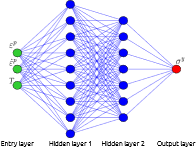
\includegraphics[width = 90 mm]{Figures/ANN}
\caption{Architecture of the ANN 3-9-7-1-sig used for the flow law}
\label{ANN}
\end{figure}

The main advantage of this approach (the use of an ANN), after the training phase, is that the output $\sigma^y$ of the network is related to the inputs $\varepsilon^p$, ${\dot{\varepsilon}}^p$, and $T$ through equations (\ref{eq:ANN-preprocess}) to (\ref{eq:ANN-vonMises}). The first step is to scale the input data to the interval $[0,1]$ using the following equation:

\begin{equation}
\overrightarrow{x} =
\begin{cases}
x_1 = \frac{\varepsilon^p - [\varepsilon^p]_{min}}{[\varepsilon^p]_{max} - [\varepsilon^p]_{min}}\\
x_2 = \frac{\ln(\mdot{\varepsilon}^p)-[\ln(\mdot{\varepsilon}^p)]_{min}}{[\ln(\mdot{\varepsilon}^p)]_{max}-[\ln(\mdot{\varepsilon}^p)]_{min}}\label{eq:ANN-preprocess}\\
x_3 = \frac{T-[T]_{min}}{[T]_{max}-[T]_{min}}
\end{cases}
\end{equation}

The outputs of the neurons in the first hidden layer are given by the following equation:

\begin{equation}
\overrightarrow{y_1} = \sigmoid\left(\w_1 \dotp \overrightarrow{x}+ \overrightarrow{b_1}\right)\label{eq:ANN-y1}
\end{equation}
where, $\sigmoid()$ is the sigmoid activation function defined by equation (\ref{eq:sigmoid}):
\begin{equation}
\sigmoid(x)=\frac{1}{1 + \e{-x}}\label{eq:sigmoid}
\end{equation}

Then, the output of the neurons in the second hidden layer are given by equation (\ref{eq:ANN-y2}):
\begin{equation}
\overrightarrow{y_2} = \sigmoid\left(\w_2 \dotp \overrightarrow{y_1}+ \overrightarrow{b_2}\right)\label{eq:ANN-y2}
\end{equation}

So, the output of the ANN is therefore given by equation (\ref{eq:ANN-vonMises}).
\begin{equation}
\sigma^y =  \left([\sigma^y]_{max}-[\sigma^y]_{min}\right) \left(\overrightarrow{w}^T \dotp \overrightarrow{y_2} + b\right) + [\sigma^y]_{min} \label{eq:ANN-vonMises}
\end{equation}

In equations (\ref{eq:ANN-preprocess}) to (\ref{eq:ANN-vonMises}), quantities $\w_1$, $\w_2$, $\overrightarrow{w}$, $\overrightarrow{b_1}$, $\overrightarrow{b_2}$ and $b$ are given by the training procedure of the ANN. Corresponding values for an ANN containing 9 neurons in the first hidden layer are reported in \ref{sec:appendix-1}. Quantities $[\ ]_{min}$ and $[\ ]_{max}$  are the boundaries of the range of the corresponding field during the training phase, values are also given in \ref{sec:appendix-1}.

Because of the large number of identified parameters for all the ANN models (from 114 to 202 for 9 and 17 neurons for the first hidden layer, respectively); the other 4 sets of ANN parameters used in this publication can be found in \cite{pantale_Coefficients_2022}.\FD{Inclure dans corps du texte puisque article normal et rq reviewer?}

\subsection{Sensitivity study of the results to mass scaling}

FE modelling of the cutting process is very expensive in CPU computation time because of the coupling fn many nonlinear phenomena and the large amount of tiny finite elements. Mass scaling (MS) is introduced in the model to reduce the CPU computation time while checking that it does not influence the results (forces and energies) via a mass scaling sensitivity study.
MS factors, ${MS}_f$, ranging from 1E6 (theoretical scaling of CPU time of $\sqrt{{MS}_f} = 1000$) to 1 (no scaling) have been used for one cutting condition ($\lambda_s$ = 0\textdegree{}, $v_c$ = 30 m/min and $h$ = 60 \textmu{}m). The same signal processing procedure is applied to the numerical forces as to the experimental forces (cf. \ref{ExpSet}): they are filtered with a second-order low-pass Bessel filter at 750 Hz before computing the mean value at steady state. Table \ref{tab:MS} gives the results normalised ($\hat{F_i}$) by these of the model without MS:
%
\begin{equation}
\hat{F_i} = \frac{F_i\text{ with MS}}{F_i\text{ without MS}}
\end{equation}
%
With $i = c$ for the cutting force and $i = f$ for the feed force. As expected, actual speed-up does not increase linearly with the ${MS}_f$, but it is still significant. ${MS}_f$ of 1E6 leads to unstable computation and ${MS}_f$ of 1E5 results in erratic forces evolutions. These results are confirmed by high values of the kinetic ($KE$) on internal ($IE$) energies ratio (it should not exceed a few \% \cite{wang_Investigation_2011, ducobu_Introduction_2015}). A ${MS}_f$ value of 1E3 is selected as it provides a good balance between computation time reduction and impact on forces, while keeping $\frac{KE}{IE}$ below 1\%. To provide an order of magnitude of CPU computation time, between 10 h and 50 h (depending on the value of $h$) are needed on 4 cores of an Intel i7-5700HQ CPU at 2.7 -- 3.5 GHz.

%
\begin{table}[!h]
\begin{center}
\caption{\label{tab:MS} MS sensitivity study (selected MS factor, $MS_f$, in bold, $\hat{F_c}$: normalized cutting force, $\hat{F_f}$: normalized feed force, $KE$: kinetic energy, $IE$: internal energy)}
\begin{tabular}{llllll}
\hline\noalign{\smallskip}
$MS_f$ & CPU scaling & Speed-up & $\hat{F_c}$ & $\hat{F_f}$ & $\frac{KE}{IE}$ (\%)\\
\noalign{\smallskip}\hline\noalign{\smallskip}
1 & 1 & 1 & 1 & 1 & 2.3E-4\\
1E2 & 10 & 9 & 1.006 & 0.982 & 2.2E-2\\
\textbf{1E3} & \textbf{32} & \textbf{21} & \textbf{1.008} & \textbf{0.940} & \textbf{2.2E-1}\\
1E4 & 100 & 61 & 1.012 & 0.921 & 2.4\\
1E5 & 316 & 173 & Erratic & Erratic & 22\\
1E6 & 1000 & 207 & Unstable & Unstable & 58\\
\noalign{\smallskip}\hline
\end{tabular}
\end{center}
\end{table}
%

\subsection{Sensitivity study of the results to the number of neurons}
\label{subsec:nberneu}

The number of neurons on the hidden layers may influence the results. A sensitivity study on the number of neurons for the first hidden layer, $\zeta$, is carried out to select the ANN providing the best balance between CPU computation time and quality of the results. The results of the study are provided in Table \ref{tab:NbNeurons}. $\check{F_i}$ corresponds to the results normalised by these of the model with the built-in JC model:
%
\begin{equation}
\check{F_i} = \frac{F_i\text{ with ANN}}{F_i\text{ with JC}}
\end{equation}
%
They show no influence on the forces when compared to the built-in Johnson-Cook model, only computation time is influenced. A first hidden layer with 9 neurons is therefore selected as it leads to the lowest CPU computation time increase.

%
\begin{table}[!h]
\begin{center}
\caption{\label{tab:NbNeurons} Sensitivity of the forces to the number of neurons of the first layer, $\zeta$
(selection in bold, $\check{F_c}$: normalized cutting force, $\check{F_f}$: normalized feed force)}
\begin{tabular}{llll}
\hline\noalign{\smallskip}
$\zeta$  & Time increase (\%) & $\check{F_c}$ & $\check{F_f}$\\
\noalign{\smallskip}\hline\noalign{\smallskip}
Built-in & 0 & 1.000 & 1.000\\
\textbf{9} & \textbf{6} & \textbf{1.000} & \textbf{0.999}\\
11 & 6 & 1.001 & 1.000\\
13 & 7 & 1.000 & 0.998\\
15 & 8 & 1.001 & 1.001\\
17 & 10 & 1.000 & 1.000\\
\noalign{\smallskip}\hline
\end{tabular}
\end{center}
\end{table}
%

%%%%%%%%%%%%%%%%%%%%%%%%%%
\section{Experimental and numerical results\label{sec:ExpNumResults}}
\label{Results}
%%%%%%%%%%%%%%%%%%%%%%%%%%

An example of temporal evolutions of numerical and experimental forces is plotted for the 3 directions in Figure \ref{ExpNum_Forces_v10_40µ_6} at $\lambda_s = 6$\textdegree{}, $v_c = 10$ m/min and $h = 40$ \textmu{}m. Computation of the FE models is carried out until a few microseconds after the steady state is reached. Then, linear extrapolation (dashed line between the two last markers in Figure \ref{ExpNum_Forces_v10_40µ_6}) is used to provide numerical values during the same time range as the experimental values. Mean and standard deviation ($2\,\sigma$) are computed from the 3 experimental values. The resulting dispersion is plotted in Figure \ref{ExpNum_Forces_v10_40µ_6} around the mean values of each forces. Steady state takes more time to be reached for the experiments than in the numerical model, and particularly for the cutting force. Dispersion around the mean force evolution is larger for the feed force than for the cutting force, while the mean feed force value is 46\% of the mean cutting force value. The numerical cutting force is very close to the experimental mean cutting force; it is only 4\% larger). This difference is computed by
%
\begin{equation}\label{eq:diff}
	\Delta i = \frac{\left|i^\text{(sim)} - i^\text{(exp)}\right|}{i^\text{(exp)}}\times 100
\end{equation}
%

 The numerical feed force is underestimated by the model, but it is at the boundary of the 95\% experimental confidence interval. The numerical passive force difference is also underestimated, but it is not in the narrower experimental dispersion. Difference between the mean values of experimental and numerical feed and passive forces is 25\%. \hl{This value for the feed force\ldots + [x] For the passive force\ldots + [x]}

\begin{figure}[!h]
\centering
\includegraphics[width = 140 mm]{Figures/ExpNum_Forces_v10_40µ_6}
\caption{Temporal evolutions of experimental (E) and numerical (N) forces at $\lambda_s = 6$\textdegree{}, $v_c = 10$ m/min and $h = 40$ \textmu{}m: dispersion around mean experimental values and linear extrapolation of numerical values in dashed}
\label{ExpNum_Forces_v10_40µ_6}
\end{figure}

Numerical chips at $v_c = 10$ m/min and $h = 40$ \textmu{}m for $\lambda_s = 0$\textdegree{} and $\lambda_s = 6$\textdegree{} are provided in Figures \ref{ChipsNum} and \ref{ChipsNumBack}. When the cutting edge inclination is 0\textdegree{}, both sides of the chip are identical and a symmetry plane can be drawn in the middle of the workpiece (Figure \ref{ChipsNumBack} (a)). On the contrary, for the cutting edge inclination of 6\textdegree{}, the chip is not aligned with the workpiece anymore. The chip bends on one side due to the orientation of the tool and the symmetry is lost for both the geometry, and the thermal and mechanical fields as highlighted in Figure \ref{ChipsNumBack} (b). This produces helical chips for the inclination angle of 6\textdegree{} as in the experiments. Figure \ref{ChipNumTop} shows the variation of the chip thickness across its width: it is thicker in the middle (i.e. the body of the chip) than on its sides. This stresses on the importance of a 3D modelling, even for the orthogonal cutting configuration as already highlighted \hl{by} \cite{Outeiro? Ambrosini? Hardt? Duco}. 3D modelling also allows to reproduce the side flow occurring in the experiments for both cutting edge inclination values (Figure \ref{ChipsNum}), contrary to a 2D \hl{model} \cite{}. Although this leads to higher computation times, future cutting models should be in 3D, even when orthogonal cutting is considered. In this case, it is recommended to take advantage of the symmetry of the configuration to reduce computation time. This simplification has not been included in this study to avoid any difference in the FE models between the 2 cutting edge inclinations.

\begin{figure}[!h]
\centering
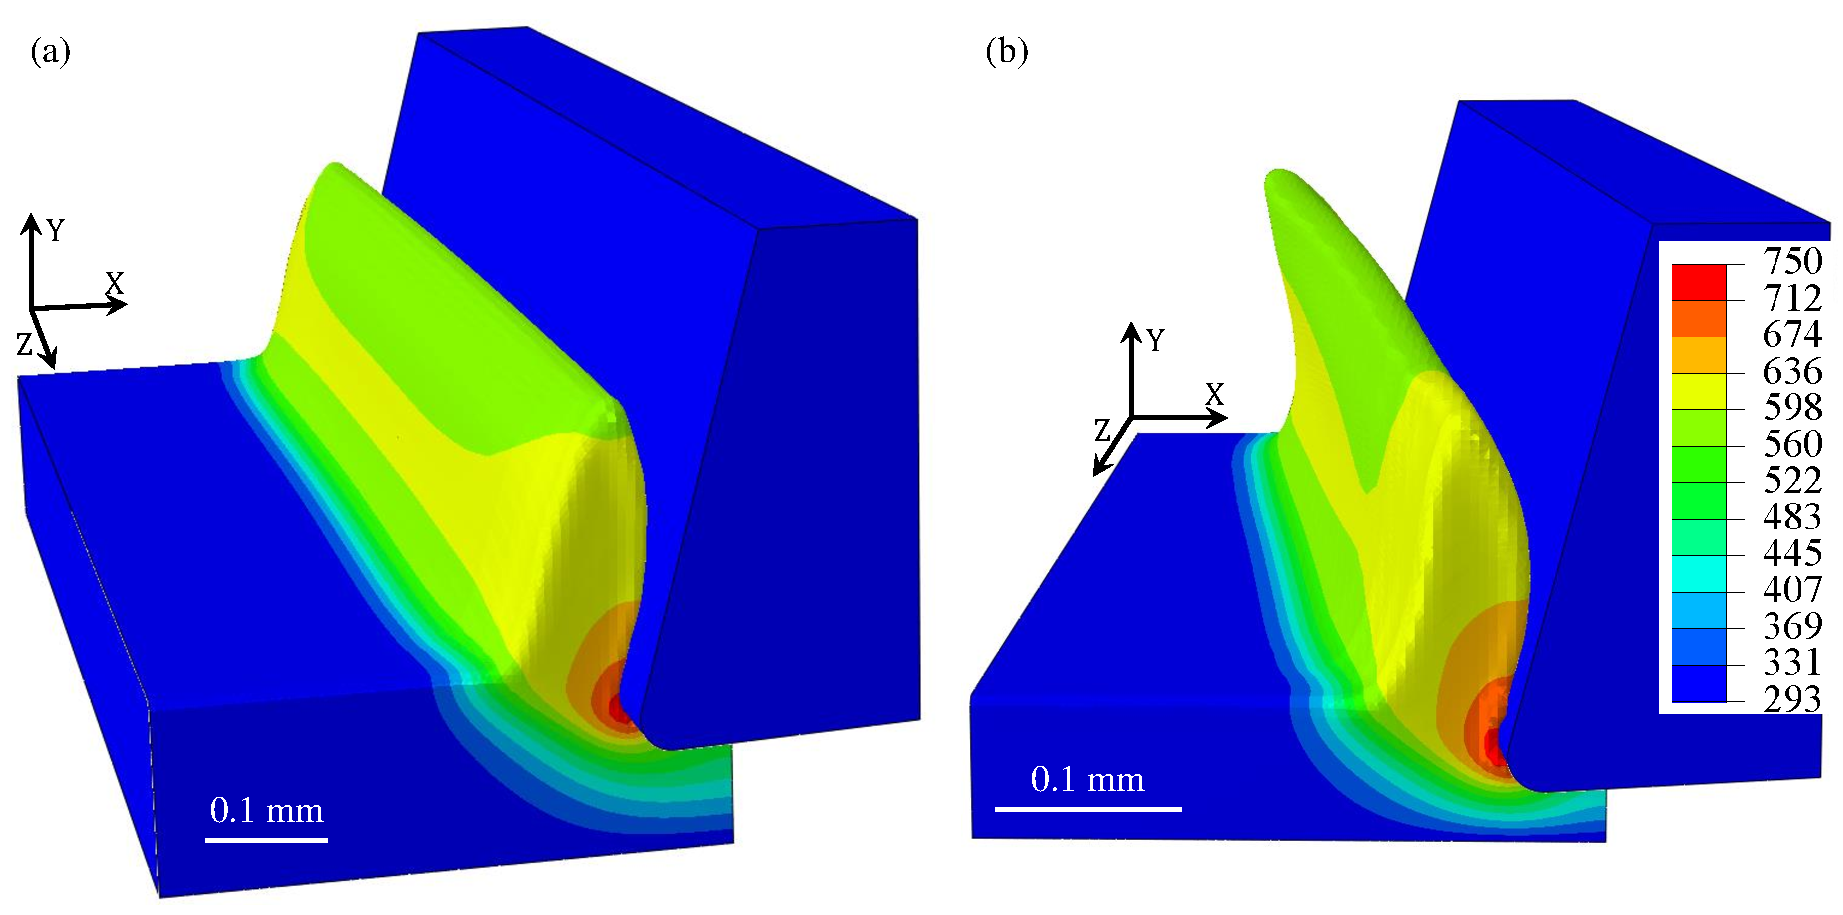
\includegraphics[width = 140 mm]{Figures/ChipsNum}
\caption{Temperature contours (in K) of the numerical chip after 1.5 ms at $v_c = 10$ m/min, $h = 40$ \textmu{}m and (a) $\lambda_s = 0$\textdegree{} and (b) $\lambda_s = 6$\textdegree{}}
\label{ChipsNum}
\end{figure}

\begin{figure}[!h]
\centering
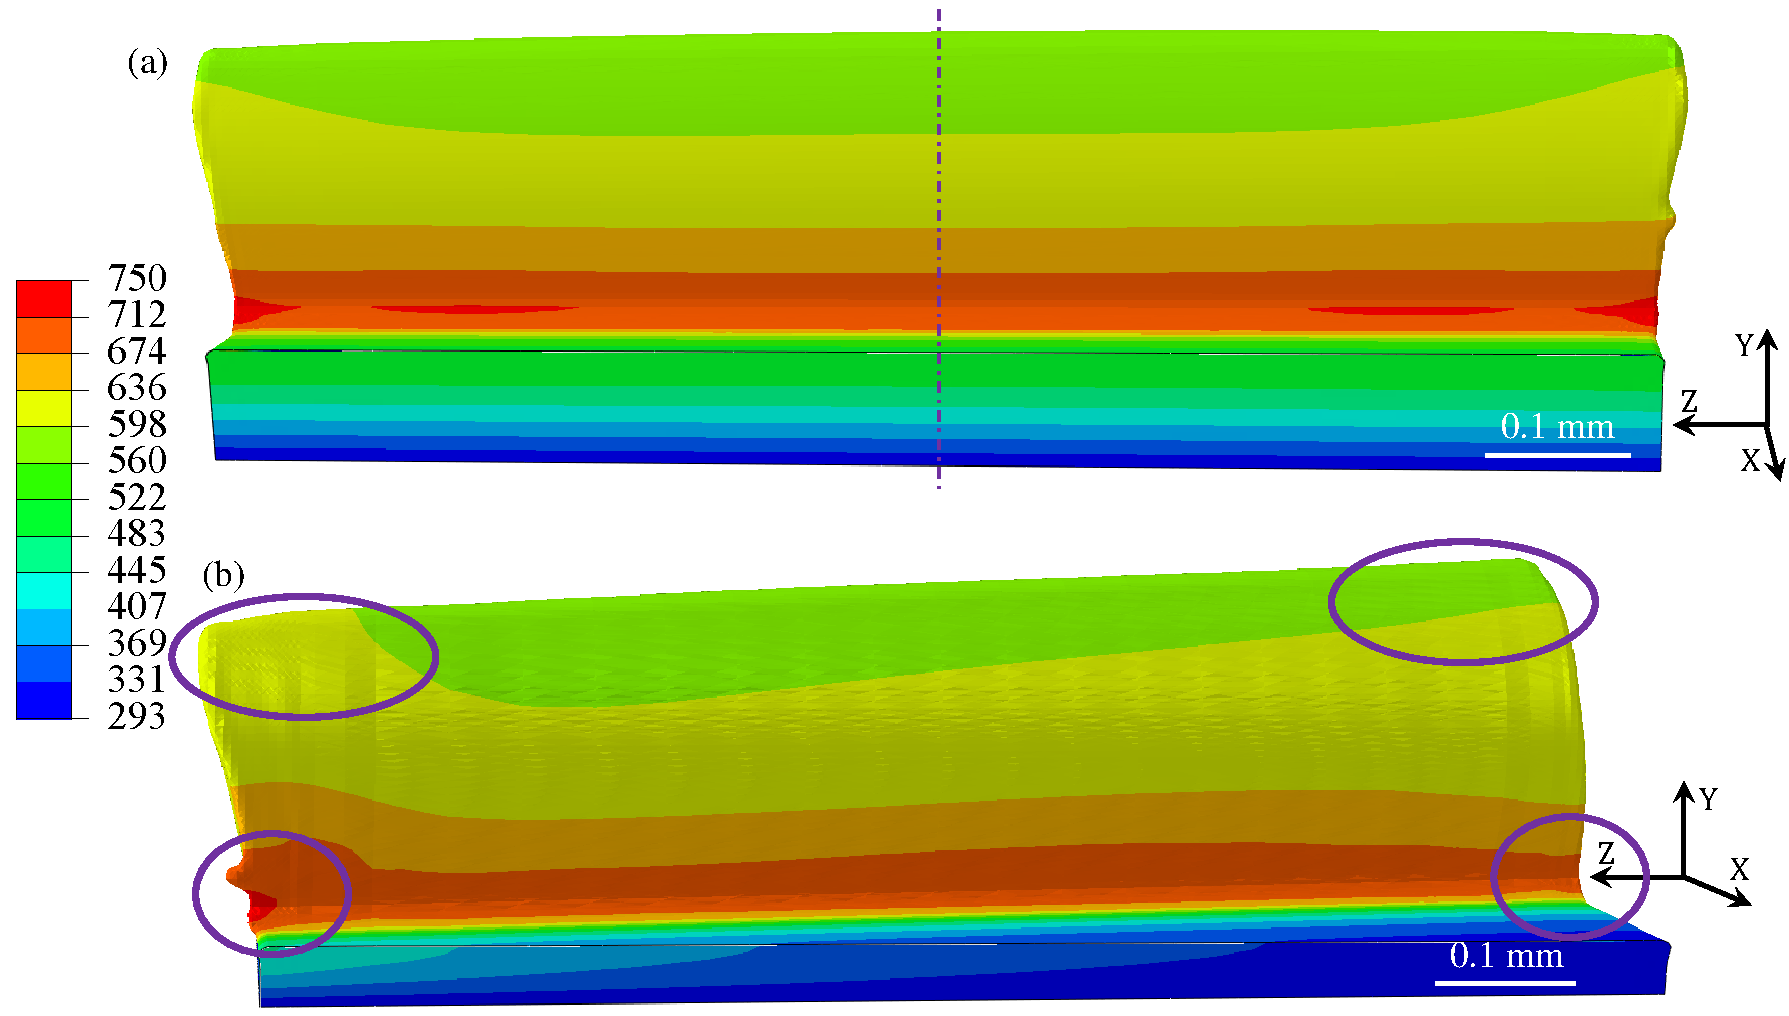
\includegraphics[width = 140 mm]{Figures/ChipsNumBack}
\caption{Temperature contours (in K) of the back of the numerical chip (tool is removed) after 1.5 ms at $v_c = 10$ m/min, $h = 40$ \textmu{}m and (a) $\lambda_s = 0$\textdegree{} and (b) $\lambda_s = 6$\textdegree{}}
\label{ChipsNumBack}
\end{figure}

\begin{figure}[!h]
\centering
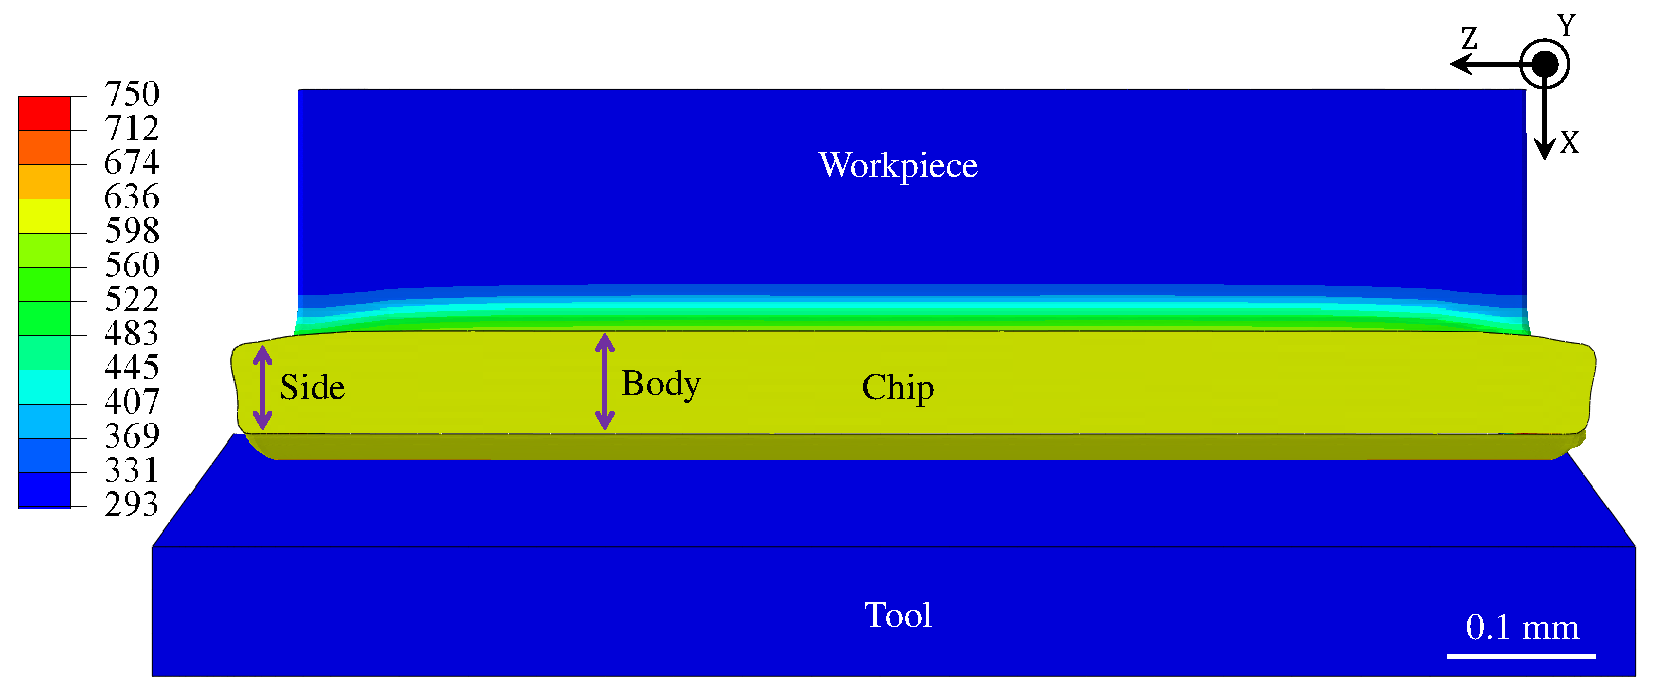
\includegraphics[width = 140 mm]{Figures/ChipNumTop}
\caption{Temperature contours (in K) of the top of the numerical chip after 1.5 ms at $v_c = 10$ m/min, $h = 40$ \textmu{}m and $\lambda_s = 0$\textdegree{}}
\label{ChipNumTop}
\end{figure}

Mean values of the experimental forces and their dispersion are shown in Figures \ref{Fx_0} to \ref{Fz_6} together with the mean numerical values. Passive force values are of course only plotted for $\lambda_s = 6$\textdegree{} as they are equal to zero when $\lambda_s = 0$\textdegree{}.

\begin{figure}[!h]
\centering
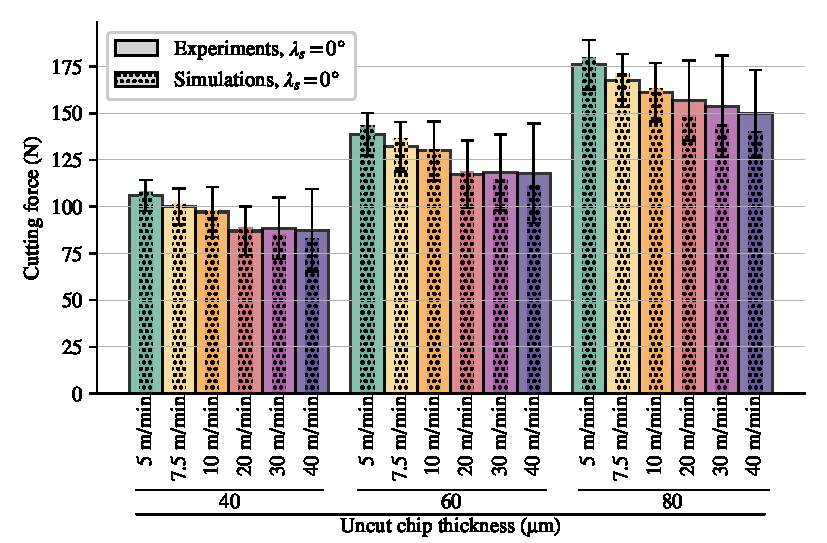
\includegraphics[width = 140 mm]{Figures/Fx_0}
\caption{Comparison of experimental (E) and numerical (N) cutting forces at the cutting edge inclination of 0\textdegree{} for the 3 uncut chip thicknesses (40, 60 and 80 \textmu{}m) and the 6 cutting speeds (5, 7.5, 10, 20, 30 and 40 m/min)}
\label{Fx_0}
\end{figure}

\begin{figure}[!h]
\centering
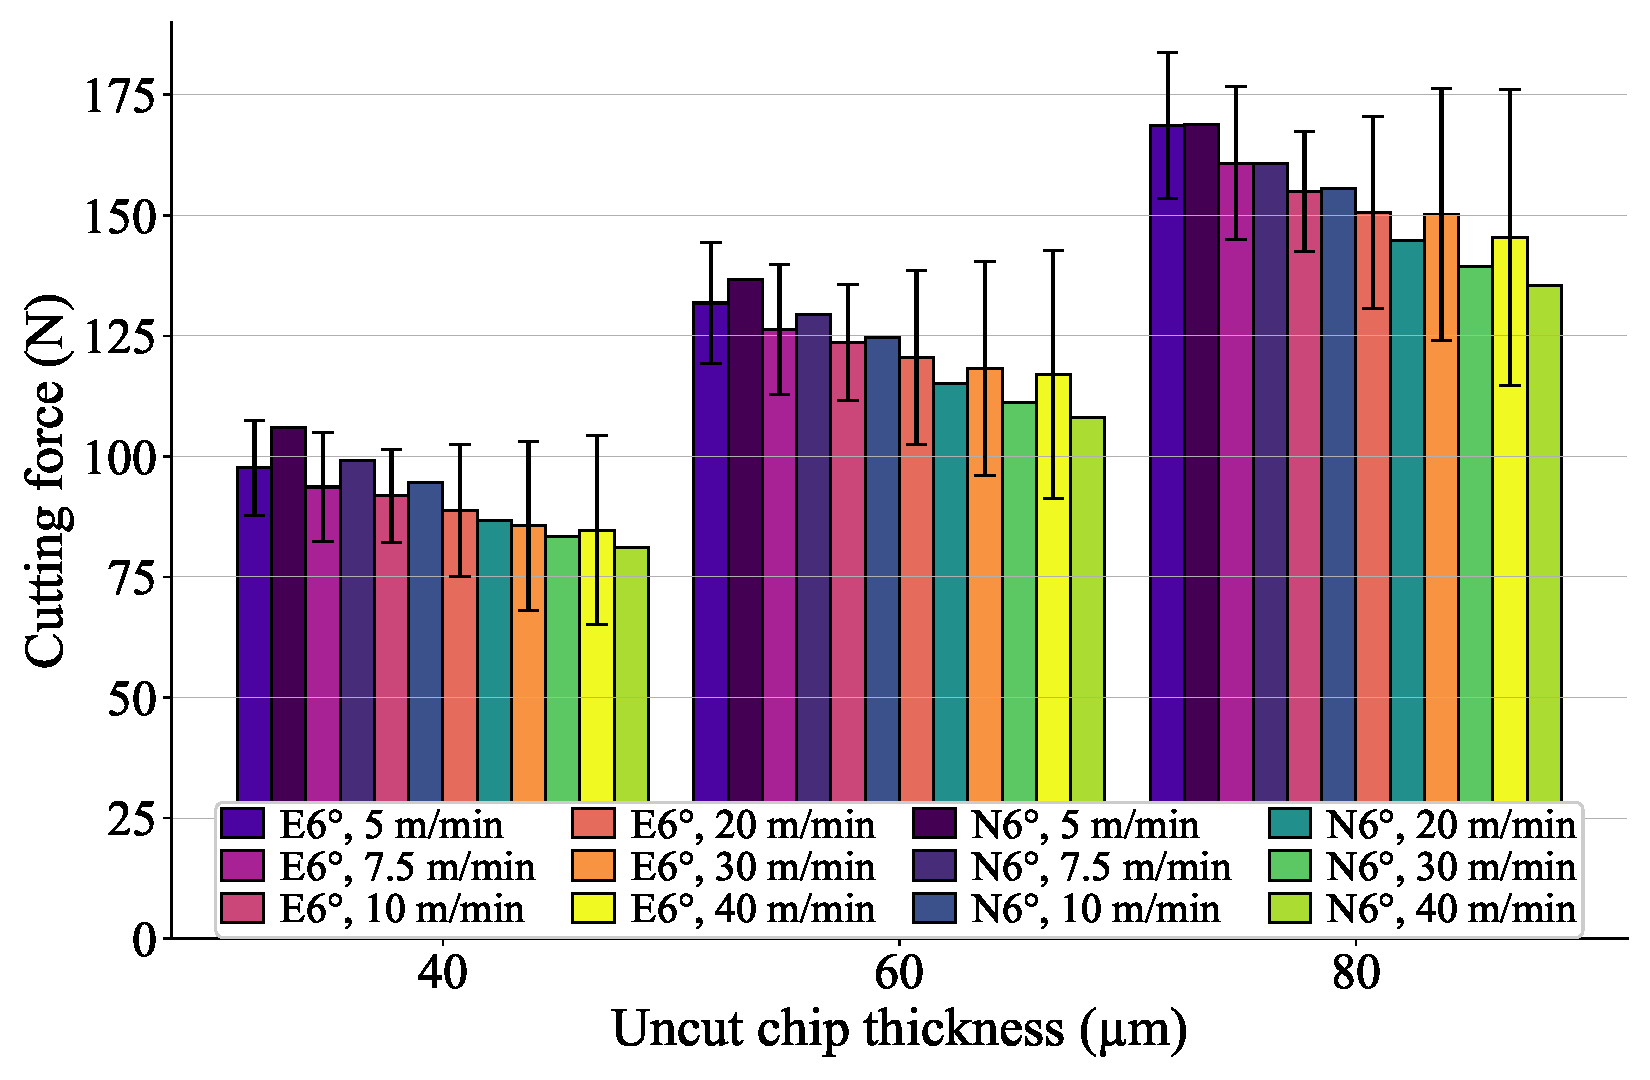
\includegraphics[width = 140 mm]{Figures/Fx_6}
\caption{Comparison of experimental (E) and numerical (N) cutting forces at the cutting edge inclination of 6\textdegree{} for the 3 uncut chip thicknesses (40, 60 and 80 \textmu{}m) and the 6 cutting speeds (5, 7.5, 10, 20, 30 and 40 m/min)}
\label{Fx_6}
\end{figure}

\begin{figure}[!h]
\centering
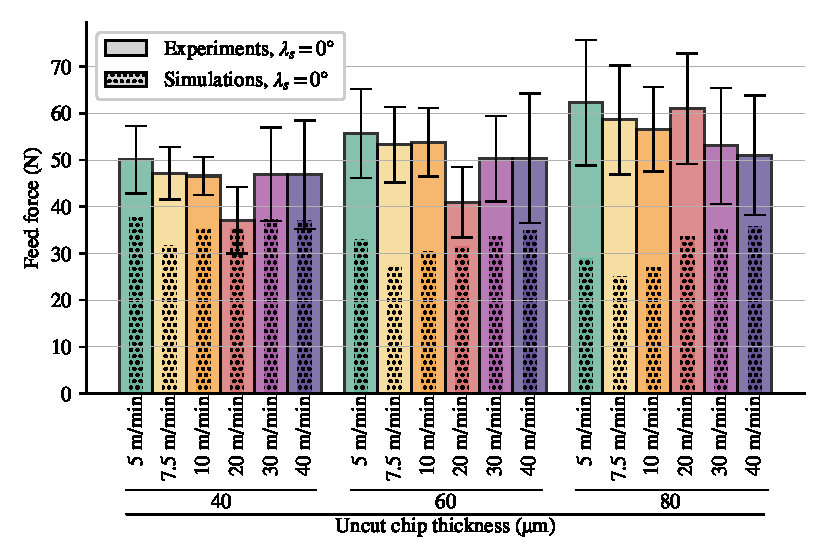
\includegraphics[width = 140 mm]{Figures/Fy_0}
\caption{Comparison of experimental (E) and numerical (N) feed forces at the cutting edge inclination of 0\textdegree{} for the 3 uncut chip thicknesses (40, 60 and 80 \textmu{}m) and the 6 cutting speeds (5, 7.5, 10, 20, 30 and 40 m/min)}
\label{Fy_0}
\end{figure}

\begin{figure}[!h]
\centering
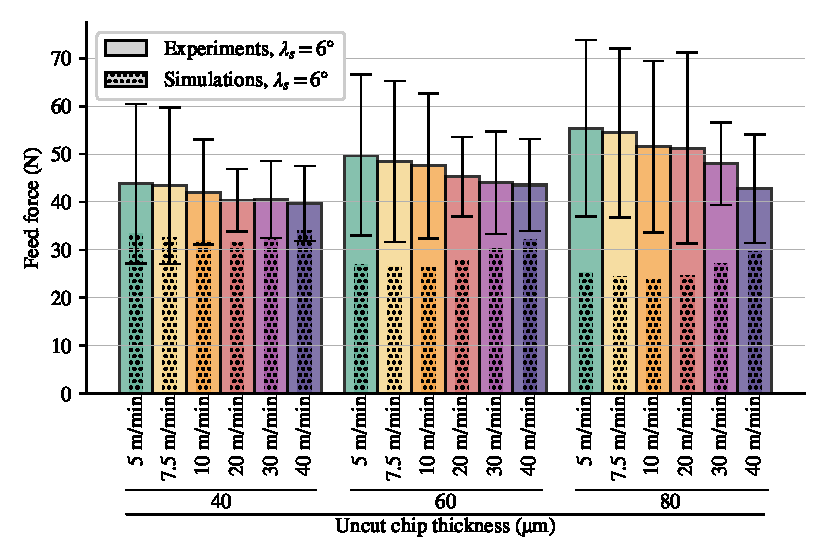
\includegraphics[width = 140 mm]{Figures/Fy_6}
\caption{Comparison of experimental (E) and numerical (N) feed forces at the cutting edge inclination of 6\textdegree{} for the 3 uncut chip thicknesses (40, 60 and 80 \textmu{}m) and the 6 cutting speeds (5, 7.5, 10, 20, 30 and 40 m/min)}
\label{Fy_6}
\end{figure}

\begin{figure}[!h]
\centering
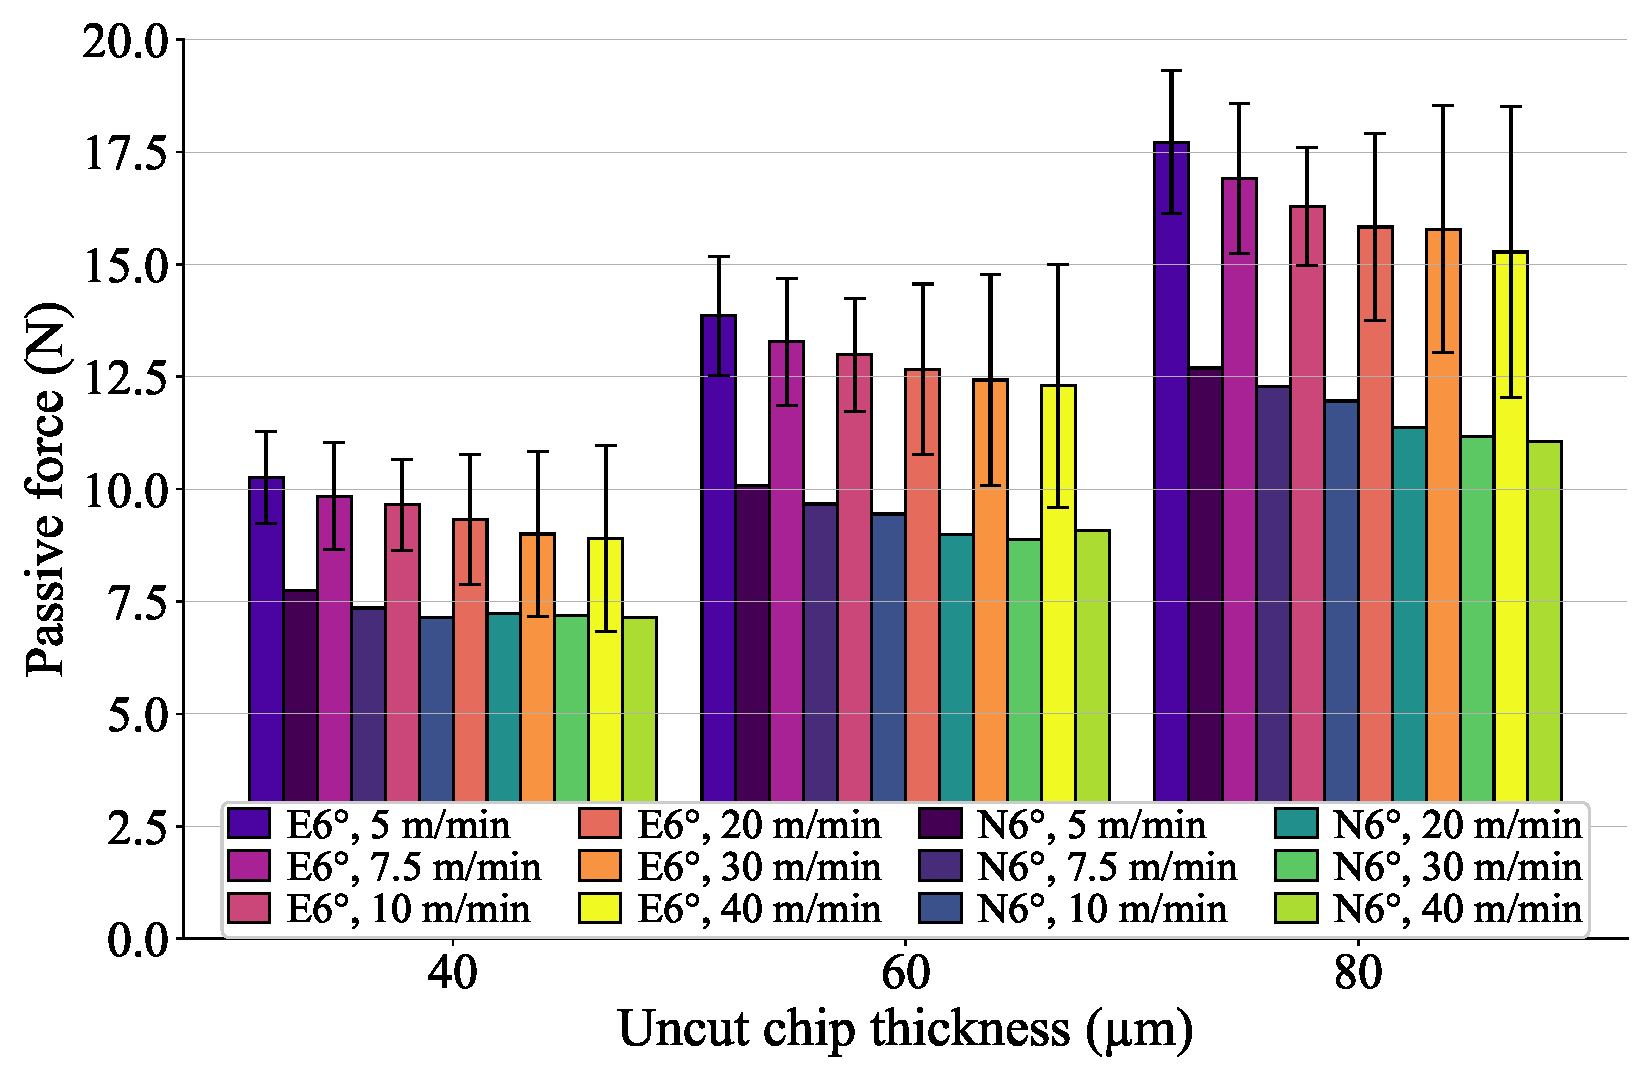
\includegraphics[width = 140 mm]{Figures/Fz_6}
\caption{Comparison of experimental (E) and numerical (N) passive forces at the cutting edge inclination of 6\textdegree{} for the 3 uncut chip thicknesses (40, 60 and 80 \textmu{}m) and the 6 cutting speeds (5, 7.5, 10, 20, 30 and 40 m/min)}
\label{Fz_6}
\end{figure}

The increase of the cutting force with the uncut chip thickness is clearly observed in Figures \ref{Fx_0} and \ref{Fx_6} for both experimental and numerical results at the 2 inclination angles, as well as the decrease of the force with the increase in the cutting speed. This shows temperature softening domination on strain rate hardening for Ti6Al4V and that it is accurately modelled. The increase of the inclination angle from 0\textdegree{} to 6\textdegree{} slightly reduces the cutting force; this is well captured by the model. For cutting speeds of 20--40 m/min and inclination angle of 0\textdegree{}, $F_c$ is almost constant with the cutting speed for uncut chip thicknesses of 40 \textmu{}m and 60 \textmu{}m, while it slightly decreases for 80 \textmu{}m; this small stabilisation is less marked for the modelling.

An increase in the deviation around the mean value with the cutting speed is noted for values above 10 m/min. All numerical values are within a confidence interval of 95\% of the experiments (35 out of 36 conditions are within a confidence interval of 68\%) and the mean difference with the experiments is 3\%, which is remarkable, moreover given the wide range of cutting conditions considered and the absence of tuning of the model. This highlights the predictive ability of the FE model for both inclination angles.

Figures \ref{Fy_0} and \ref{Fy_6} show the results for the feed force, where the two clearest trends for the experiments are its decrease with inclination angle and its increase with the uncut chip thickness (even if it is smaller that the expectations). For 80 \textmu{}m, $F_f$ globally decreases with $v_c$ in the experiments. For 40 \textmu{}m and 60 \textmu{}m, the force decreases at lower $v_c$ and then increases for 0\textdegree{}, while a decrease is observed at all $v_c$ for 6\textdegree{}. For the numerical values, the global trend is the same for the 3 uncut chip thicknesses and both inclination angles: a decrease for the lowest $v_c$ values and then an increase. It must be noted that the numerical model does not handle correctly the feed force trends: as clearly shown by Figure \ref{Fy_6}, the numerical forces have globally an increasing trend with the cutting speed, while their mean value mostly decreases when the uncut chip thickness increases. Differences between the mean numerical and experimental values increase with the uncut chip thickness: forces are closer at 40 \textmu{}m than at 80 \textmu{}m. The numerical values are mostly not within the 95\% confidence interval (it has no clear evolution with the cutting conditions). Coupled with the differences in trends, it shows that $F_f$ is less well modelled (mean difference is 35\%) than $F_c$ as usual in FE modelling of the cutting \hl{process} \cite{}. The influence of the uncut chip thickness on the feed force should therefore be improved. Material constitutive model parameters are known to have an impact on the forces (and on the chip \hl{morphology)} \cite{duco}. The friction model should be improved as well to enhance the results.

Passive force is non-zero for the inclination angle of 6\textdegree{} (Figure \ref{Fz_6}). As the cutting force, it increases with the uncut chip thickness and it decreases with the cutting speed. Comparison with the experiments is globally the same as for $F_c$, except for a larger difference in the magnitude of $F_p$ (mean difference is 26\%, but it is small in absolute – less than 5 N). The numerical values are mostly not in the 95\% experimental confidence interval.

Regarding the chips morphology, all the chips are continuous. For both the simulation and the experiments, the chip thickness ratio, $\lambda_h$:
\begin{equation}
\lambda_h = \frac{h'}{h}
\end{equation}
with $h$ the uncut chip thickness and $h'$ the chip thickness, is almost independent of the uncut chip thickness. It is slightly reduced from $\lambda_s = 0$\textdegree{} to $\lambda_s = 6$\textdegree{}, meaning that the chip thickness is reduced with the inclination angle. This influence is underestimated by the model: the reduction of $\lambda_h$ is lower than in the experiments. The mean difference between experimental and numerical $\lambda_h$ is 17\% across the whole range of cutting conditions. The chip thickness ratio decreases with the cutting speed because of the reduction of friction, which is correctly captured by the model. As for the feed force, the results should be improved by more complex friction models and a set of material constitutive parameters for which the identification includes the forces and the chip thickness \cite{kugalurpalanisamy_Identification_2022}.

\begin{figure}[!h]
\centering
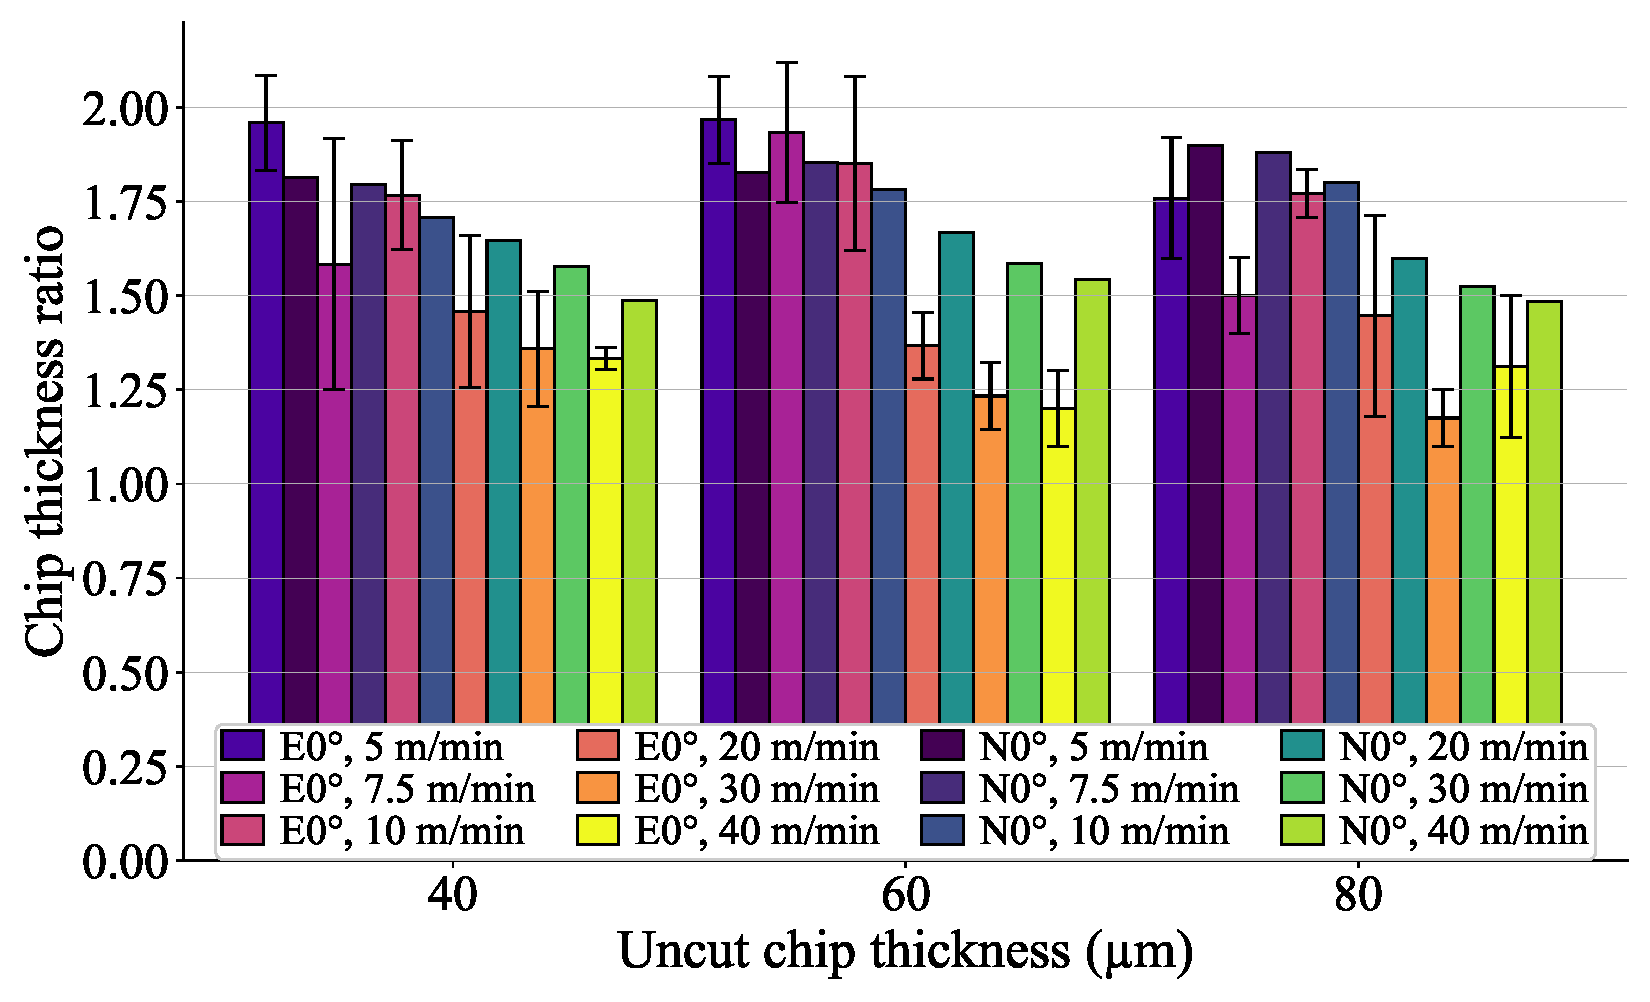
\includegraphics[width = 140 mm]{Figures/h0}
\caption{Comparison of experimental (E) and numerical (N) chip thickness ratios at the cutting edge inclination of 0\textdegree{} for the 3 uncut chip thicknesses (40, 60 and 80 \textmu{}m) and the 6 cutting speeds (5, 7.5, 10, 20, 30 and 40 m/min)}
\label{h0}
\end{figure}

\begin{figure}[!h]
\centering
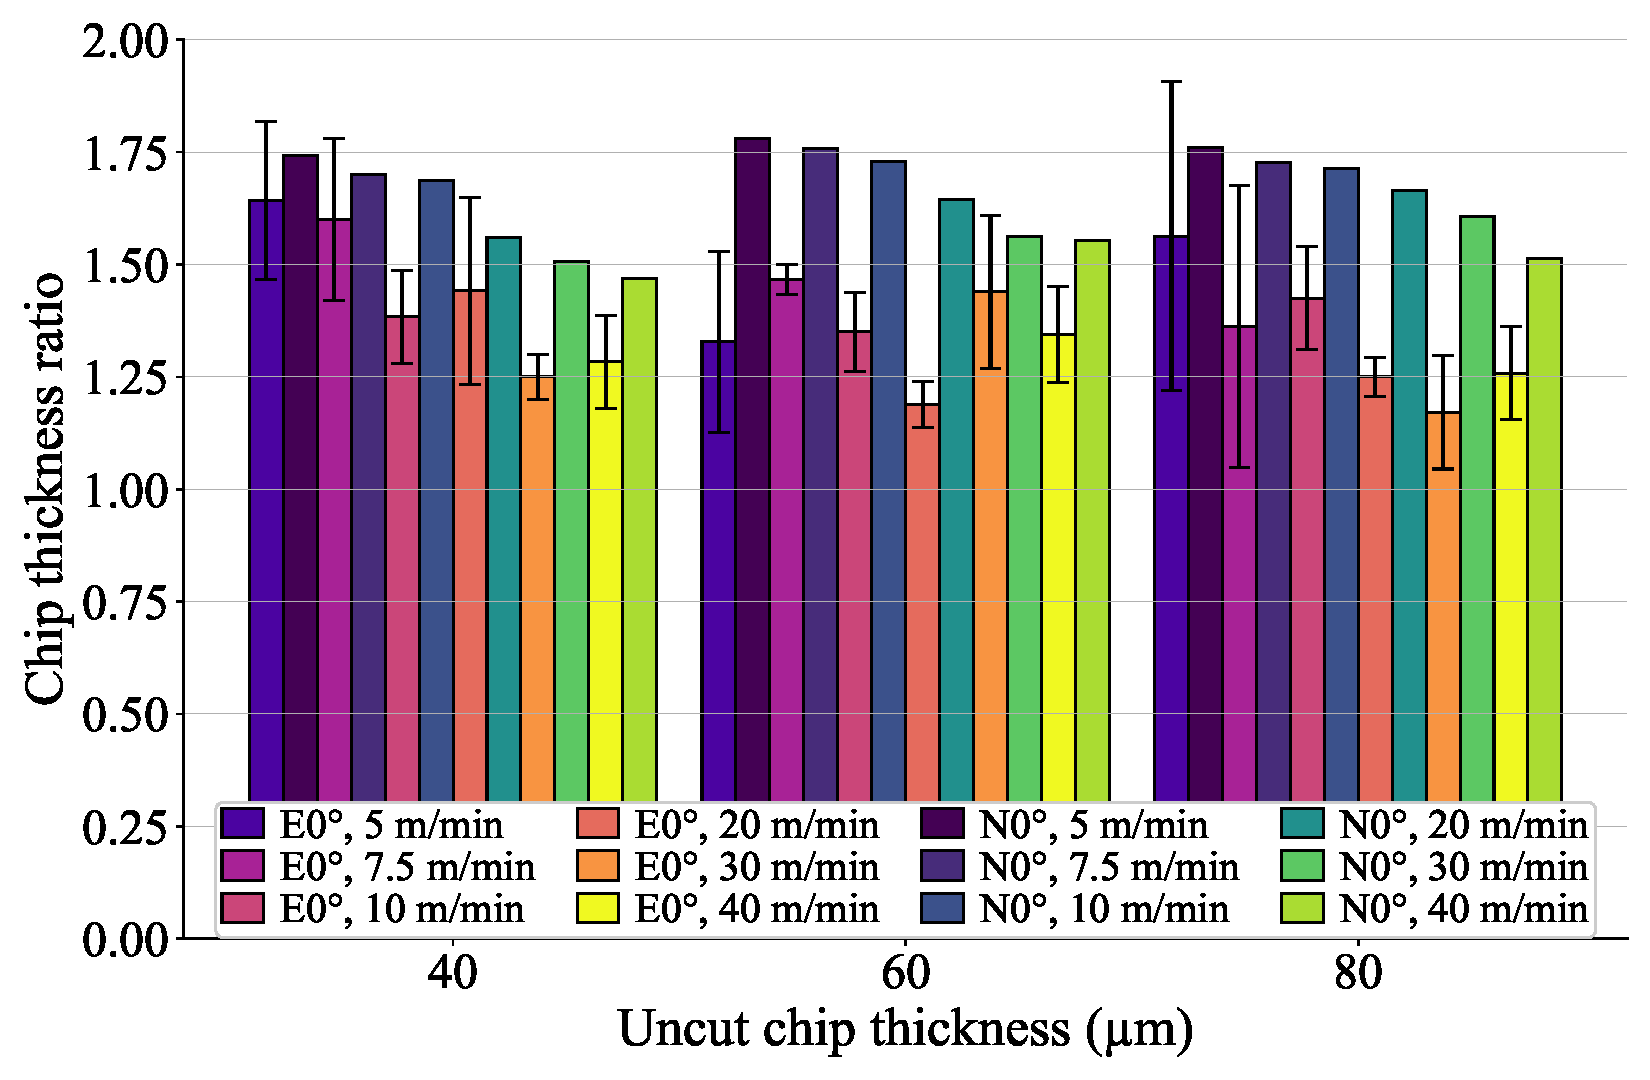
\includegraphics[width = 140 mm]{Figures/h6}
\caption{Comparison of experimental (E) and numerical (N) chip thickness ratios at the cutting edge inclination of 6\textdegree{} for the 3 uncut chip thicknesses (40, 60 and 80 \textmu{}m) and the 6 cutting speeds (5, 7.5, 10, 20, 30 and 40 m/min)}
\label{h6}
\end{figure}

Differences computed according to equation \ref{eq:diff} \hl{+ comment} and link to Table \ref{tab:Synth}

%
\begin{table}[!h]
\begin{center}
\caption{\label{tab:Synth} Synthetic overview of the results: differences between the experimental and the numerical results (mean difference for each cutting edge inclination, and maximal, minimal and mean differences for all the conditions) for the cutting force, $\Delta F_c$, the feed force, $\Delta F_f$, the passive force, $\Delta F_p$, and the chip thickness ratio, $\Delta \lambda_h$}
\begin{tabular}{lllll}
\hline\noalign{\smallskip}
Difference & $\Delta F_c$ (\%) & $\Delta F_f$ (\%) & $\Delta F_p$ (\%) & $\Delta \lambda_h$ (\%)\\
\hline\noalign{\smallskip}
Mean $\lambda_s = 0$\textdegree{} & 3 & 38 & -- & 14\\
Mean $\lambda_s = 6$\textdegree{} & 4 & 40 & 26 & 21\\
Max global & 10 & 60 & 29 & 38\\
Min global & 1 & 10 & 19 & 2\\
Mean global & 4 & 39 & 26 & 17\\
\noalign{\smallskip}\hline\noalign{\smallskip}
\end{tabular}
\end{center}
\end{table}
%

%%%%%%%%%%%%%%%%%%%%%%%%%%
\section{Conclusions}
%%%%%%%%%%%%%%%%%%%%%%%%%%

In this paper, an experimental study has been carried out in free orthogonal and oblique cutting of the titanium alloy Ti6Al4V. It is a reference to assess the performances of the 3D FE model introducing an ANN-based constitutive model and developed in the same conditions. An unpreviously seen wide range of cutting conditions, 36, is considered, including 2 cutting edge inclinations. Accurate evaluation of fundamental variables in 3D with the absence of tuning of both numerical parameters and model features when cutting conditions and inclination angle are significantly modified is a strong novelty of this work. Only changing the inclination angle to move from free orthogonal to oblique cutting while maintaining the quality of the results has no equivalent in the current literature, moreover as no study on free oblique cutting is available. Predictive abilities of the model make it adequate for development of tools with a straight cutting edge, for example, providing the modelling of the feed force is improved if it is relevant for the study. This work moreover demonstrates the ability to model materials behaviour with ANN and opens possibilities in this promising direction.

%%%%%%%%%%%%%%%%%%%%%%%%%%
%%% References
%%%%%%%%%%%%%%%%%%%%%%%%%%
%%%
%%% Following citation commands can be used in the body text:
%%% Usage of \cite is as follows:
%%%   \cite{key}          ==>>  [#]
%%%   \cite[chap. 2]{key} ==>>  [#, chap. 2]
%%%   \citet{key}         ==>>  Author [#]
%
%%% References with bibTeX database:
%
\bibliographystyle{model1-num-names}
\bibliography{Biblio}
%
%%% Authors are advised to submit their bibtex database files. They are
%%% requested to list a bibtex style file in the manuscript if they do
%%% not want to use model1-num-names.bst.
%
%%% References without bibTeX database:
%
%% \begin{thebibliography}{00}
%


%%% \bibitem must have the following form:
%%%   \bibitem{key}...
%%%
%
%% \bibitem{}
%
%% \end{thebibliography}
%

%%%%%%%%%%%%%%%%%%%%%%%%%%%
%%% The Appendices part is started with the command \appendix;
%%% appendix sections are then done as normal sections
\appendix
%
\section{Coefficients of the ANN 3-9-7-1-sig\label{sec:appendix-1}}

In this Appendix, we present the values obtained after the training phase of an ANN containing 9 neurons in the first hidden layer and 7 neurons in the second hidden layer.

The training of the neural network was performed using a data set containing $3\,430$ data points defined by:
\begin{itemize}
\item $70$ values for $\varepsilon^p\in[0.0,3.0]$, so that $[\varepsilon^p]_{min}=0$ and $[\varepsilon^p]_{max}=3$.
\item $7$ plastic strain rates $\mdot{\varepsilon}^p\in[1, 10, 50, 500, 5\,000, 50\,000, 500\,000]$, so that $[\ln(\mdot{\varepsilon}^p)]_{min}=0$ and $[\ln(\mdot{\varepsilon}^p)]_{max}=13.12236$. \FD{Add units to values?}
\item  $7$ temperatures $T\in[293, 400, 500, 700, 900, 1\,200, 1\,500]$, so that $[T]_{min}=293$ and $[T]_{max}=1\ 500$. \FD{Add units to values?}
\end{itemize}

Stresses in the training dataset ranges from $[\sigma^y]_{min}=171.44$ to $[\sigma^y]_{max}=2606.12$.
The results of the training process are given below for quantities $\w_1$, $\w_2$, $\overrightarrow{w}$, $\overrightarrow{b_1}$, $\overrightarrow{b_2}$ and $b$.

\begin{equation*}
\w_1=\left[
\begin{array}{rrr}
 -0.87229 & -0.47675 & -1.50771\\
 -0.95762 & -0.25619 &  1.65222\\
 -10.61660 &  0.22003 & -0.11539\\
  3.67883 &  0.37146 & -1.51069\\
 -63.39468 &  0.15466 & -0.95431\\
  0.54807 &  0.25959 & -5.44355\\
 -1.33883 &  0.36089 & -1.66735\\
 -0.68125 &  1.02121 &  0.34242\\
  0.08740 &  0.18764 & -41.32542
\end{array}\right]
\end{equation*}

\begin{equation*}
\w_2^T=\left[
\begin{array}{rrrrrrrrr}
  1.66285 & -0.59645 & -3.17333 &  0.20706 &  1.18760 &  2.01250 & -0.82147\\
 -0.26237 & -2.50330 & -1.45941 & -1.59833 &  4.05169 & -1.21146 &  1.05610\\
 -0.12958 &  0.67119 & -5.85989 & -2.55061 &  4.85245 &  4.31876 &  3.24070\\
 -2.12890 &  0.68296 &  0.71183 &  0.81706 & -0.09405 &  0.34919 & -1.41223\\
  2.33631 & -0.08089 &  14.65789 &  0.12531 &  23.66363 &  2.55872 &  2.15338\\
  0.11567 &  1.77629 & -1.80448 &  0.77825 & -1.58254 &  1.90442 &  1.23152\\
  1.49265 &  0.41821 & -3.53803 & -0.48705 & -0.23671 &  0.75887 & -0.37441\\
  0.95990 &  0.69041 &  0.43870 &  0.28393 & -1.40101 & -0.64569 & -0.38964\\
  5.89937 & -0.13015 &  2.99264 &  1.78534 & -3.90189 &  1.17494 & -3.78854
\end{array}\right]
\end{equation*}

\begin{equation*}
\overrightarrow{w}=\left[
\begin{array}{r}
  0.34701\\
  1.42079\\
 -0.96564\\
  0.62467\\
 -0.56322\\
  0.40960\\
 -0.42810
\end{array}\right]
\end{equation*}

\begin{equation*}
\overrightarrow{b_1}=\left[
\begin{array}{r}
  2.57141\\
  0.22673\\
 -1.16985\\
 -0.11246\\
 -0.82210\\
 -2.13264\\
  0.78794\\
  1.20434\\
 -3.48681
\end{array}\right]
\end{equation*}

\begin{equation*}
\overrightarrow{b_2}=\left[
\begin{array}{r}
 -0.36566\\
 -1.14445\\
 -0.79065\\
 -0.50670\\
  1.30136\\
  0.04521\\
 -0.29995
\end{array}\right]
\end{equation*}

\begin{equation*}
b=0.04213
\end{equation*}

%%% \section{}
%%% \label{}
%

\end{document}
